\documentclass[12pt,a4paper]{article}
\usepackage{graphicx}
\usepackage{amsmath}
\setlength{\topmargin}{0cm}

\begin{document}
\title{notaR - um sistema para notas automatizadas em cursos que utilizam
	a linguagem R}
\author{Andre Chalom}
\maketitle

\begin{abstract}
O notaR \'e um sistema para corre\c c\~ao autom\'atica de exerc\'icios em
linguagem R, armazenamento e visualiza\c c\~ao das notas resultantes. Ele
\'e um software colaborativo, desenvolvido em linguagens de c\'odigo aberto.
\end{abstract}
\section{Perfis de acesso}
O sistema pode ser acessado por:
\begin{enumerate}
	\item Professor: Pode cadastrar exerc\'icios, e ver relat\'orios como
			notas por aluno, exerc\'icios com mais dificuldades, etc,
	\item Aluno: Pode submeter exerc\'icios e ver tabelas com as pr\'oprias
			notas recebidas anteriormente,
	\item Ouvinte: Pode submeter exerc\'icios, mas sua nota n\~ao \'e
			gravada no sistema
\end{enumerate}
\begin{figure}[htbp]
		\begin{center}
				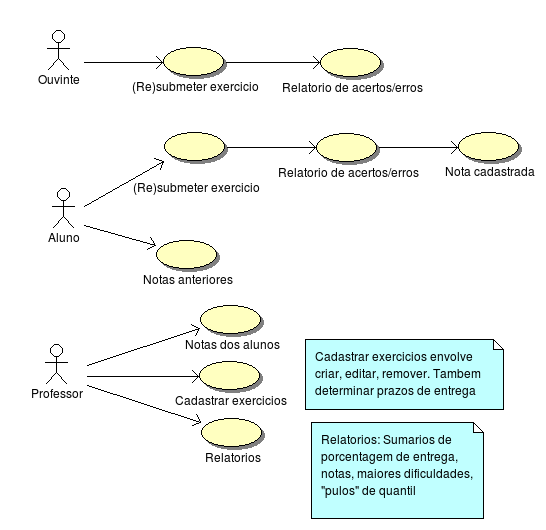
\includegraphics[scale=0.50]{model/utilizacao.png}
		\end{center}
		\caption{Perfis de utiliza\c c\~ao}
		\label{fig:utilizacao}
\end{figure}
\section{M\'odulos}
O sistema \'e composto pelos seguintes m\'odulos:
\begin{enumerate}
	\item Visualiza\c c\~ao: escrito em PHP como plug-in para o Dokuwiki
	\item Processamento: escrito em R, \'e quem realiza a corre\c c\~ao de
			exerc\'icios propriamente dita
	\item Dados: banco em MySQL
\end{enumerate}

\begin{figure}[htpb]
		\begin{center}
				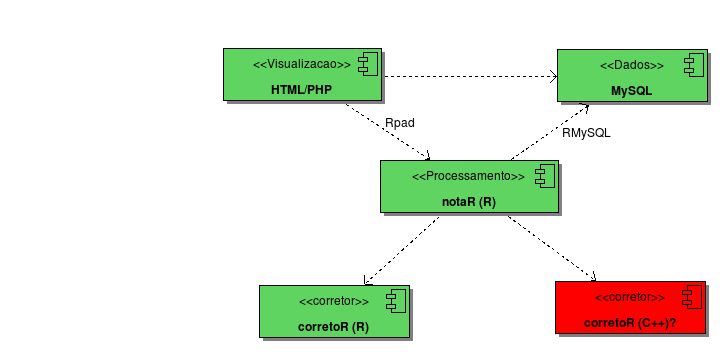
\includegraphics[scale=0.50]{model/modulos.png}
		\end{center}
		\caption{Esquema dos m\'odulos do sistema}
		\label{fig:modulos}
\end{figure}
\section{Instala\c c\~ao}
Para utilizar o notaR em um curso, s\~ao necess\'arios os seguintes passos:
\begin{enumerate}
	\item Instala\c c\~ao do software de suporte (Dokuwiki, MySQL, R),
	\item Instala\c c\~ao do notaR em si,
	\item Prepara\c c\~ao e cadastramento dos exerc\'icios no notaR.
\end{enumerate}

\end{document}
